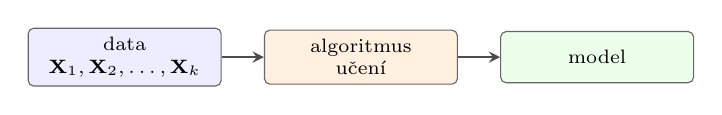
\begin{tikzpicture}[
    >=stealth,
    box/.style={
        draw=black!60,
        rounded corners=2pt,
        minimum width=2.45cm,
        minimum height=0.65cm,
        align=center,
        font=\scriptsize
    },
    arr/.style={->, thick, draw=black!70}
]
    \node[box, fill=blue!7] (data) at (0,0)
        {data\\$\mathbf{X}_1,\mathbf{X}_2,\dots,\mathbf{X}_k$};

    \node[box, fill=orange!12] (learn) at (3.0,0)
        {algoritmus\\učení};

    \node[box, fill=green!8] (model) at (6.0,0)
        {model};

    \draw[arr] (data) -- (learn);
    \draw[arr] (learn) -- (model);
\end{tikzpicture}
